\tp{V�rification exp�rimentale\\
de la deuxi�me loi de Newton dans\\
le cas d'une trajectoire parabolique
}


\objectifs{
\item V�rifier que le vecteur $\vect{\Delta V}$ est colin�aire et de m�me
  sens que la force appliqu�e � un solide.
}

\materiel{
\item cam�ra vid�o
\item t�l�viseur
\item magn�toscope
\item papier calque
}


\vressort{3}

\section{Protocole}

\begin{enumerate}

\item \`A l'aide d'une cam�ra vid�o, enregistrer le mouvement d'une balle de
golf lanc�e dans un plan frontal, c'est � dire dans un plan
perpendiculaire � l'axe de vis�e de la cam�ra.

\item \`A l'aide d'un magn�toscope, faire d�filer l'enregistrement
  image par image et pointer le centre de la balle sur le transparent
  coll� sur l'�cran du t�l�viseur.

\end{enumerate}


\vressort{3}

\begin{center}

\begin{figure}[H]
%\fig{9cm}{6.5cm}{}
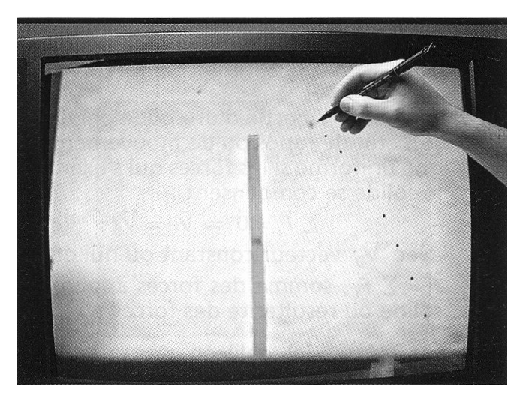
\includegraphics[width=15cm]{tp_prem_s_phys/tp08_deuxieme_loi_newton_parabole_video/2newton_tv.png.eps}

\caption[2newton_tv]{Rep�rage sur l'�cran et trac� sur papier calque des positions enregistr�es de la balle de golf}
\end{figure}

\end{center}


\vressort{1}


\newpage

\section{Exploitation de l'enregistrement}
\`A partir du transparent, d�terminer :

\indent
\begin{itemize}
\item la vitesse instantan�e en chacune des positions enregistr�es
\item le vecteur $\vect{\Delta V} = \vect{V_j} - \vect{V_i}$,
  correspondant � deux positions cons�cutives $i$ et $j$ de la balle.
\end{itemize}


\vressort{1}

\begin{enumerate}
\item \'Enoncer la deuxi�me loi de Newton.
\item Effectuer l'inventaire des forces agissant sur la balle de golf.
\item Indiquer la cons�quence de la deuxi�me loi de Newton et comparer
  avec les faits exp�rimentaux observ�s.
\end{enumerate}


\vressort{3}


\begin{center}
% Enregistrement du mouvement d'une balle de golf
%\hspace*{-1cm}\fig{18cm}{15cm}{}
\begin{figure}[H]
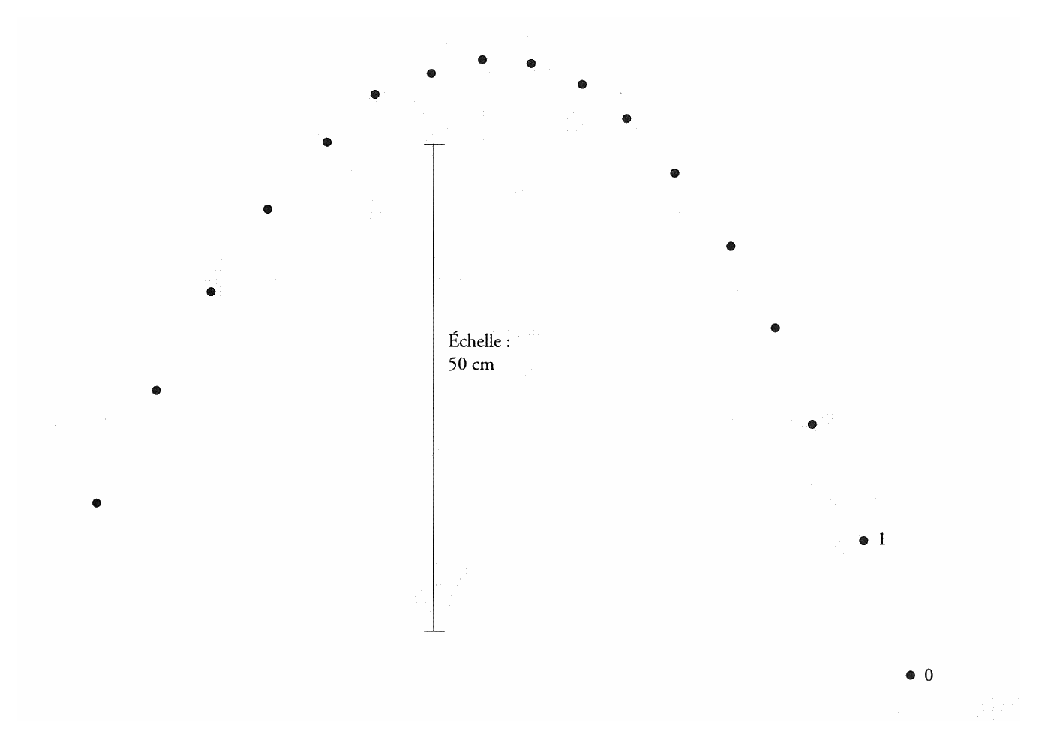
\includegraphics[width=16cm]{tp_prem_s_phys/tp08_deuxieme_loi_newton_parabole_video/2newton_traj_parabo.png.eps}

\caption[2newton_traj_parabo]{Enregistrement du mouvement d'une balle de golf}
\end{figure}

\end{center}


\vressort{1}

